\section{Versione mobile}

Non c'è nessuna versione mobile del sito. Ho deciso tuttavia di parlarne in questa sezione
perchè, in un mondo in cui ormai l'utilizzo del web da un dispositivo mobile ha superato
quello desktop, è inaccettabile non ci sia almeno un \emph{layout fluido}.
Inoltre, il sito torna utile durante le \emph{sessioni di gioco} (dove ci si riunisce con
gli amici per giocare effettivamente ad esso), una risorsa online da controllare
torna estremamente utile. E certamente, nessuno dei giocatori disporrà di un portatile a testa,
dovendo consultare il sito in versione desktop da uno smartphone e continuare a scrollare a destra e sinistra
ad ogni riga per poter leggere tutto.

La schermata che attenderà l'utente, \emph{in ogni singola} pagina, sarà il seguente. Praticamente l'intera schermata occupata dal
logo del sito.

\begin{figure}[hbt]
    \centering
    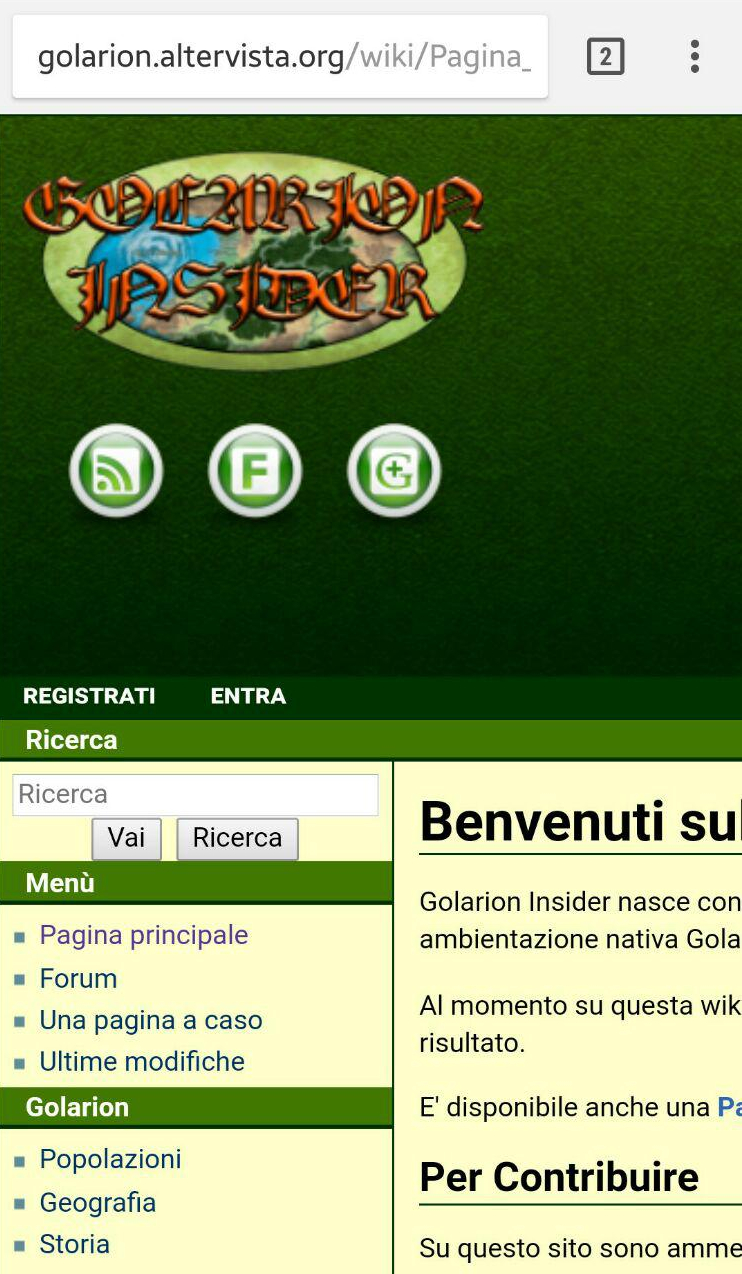
\includegraphics[width=0.5\textwidth]{img/mobile.jpg}
    \caption{Layout ``mobile'', \href{http://golarion.altervista.org/wiki/Pagina_principale}{Homepage - Golarion Insider}}
\end{figure} 

Non penso ci sia molto altro da commentare, se non sottolineare che è estremamente scomodo e rende il sito 
da mobile al limite dell'inutilizzabile.
